\chapter{Einleitung}

\textit{Umgang mit grammatikalischen Geschlechtern: Aus Gründen der Spracheleganz wird vor allem die männliche Form (zum Beispiel "`Benutzer"') verwendet. Die weibliche Form ist jedoch sinngemäss mitgemeint.}

\section{Blabla}



Hier ein Beispiel für eine Referenz zu einem Buch \cite{viz}. 



So macht man ein Text Zitat \textit{The Eyes Have It: A Task by Data Type for Information Visualizations} von B. Shneiderman \cite{shneiderman}. 


So verweisst man auf eine Abbildung \ref{fig:nytimes-taxes}.

\begin{figure}[H]
	\centering
	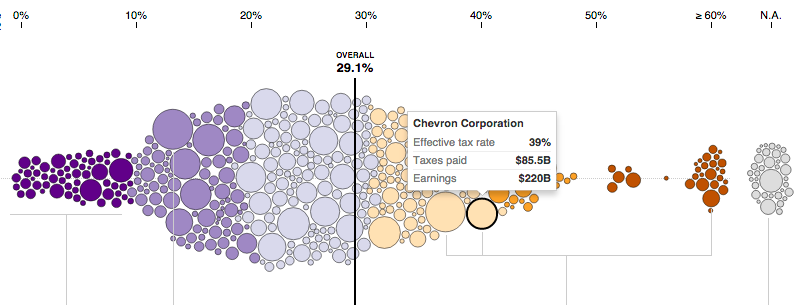
\includegraphics[width=\linewidth]{images/nytimes-taxes-zugeschnitten}
	\caption[Blasendiagramm in The New York Times (\citedate{nytimes-taxes})]{Ein Blasendiagramm, das Steuerabgaben und Steuersätze von US-Firmen darstellt. \cite{nytimes-taxes}}
	\label{fig:nytimes-taxes}% das braucht man um darauf zu verweisen
\end{figure}
